\documentclass{ximera}

%\usepackage{todonotes}

\newcommand{\todo}{}

\usepackage{esint} % for \oiint
\ifxake%%https://math.meta.stackexchange.com/questions/9973/how-do-you-render-a-closed-surface-double-integral
\renewcommand{\oiint}{{\large\bigcirc}\kern-1.56em\iint}
\fi


\graphicspath{
  {./}
  {ximeraTutorial/}
  {basicPhilosophy/}
  {functionsOfSeveralVariables/}
  {normalVectors/}
  {lagrangeMultipliers/}
  {vectorFields/}
  {greensTheorem/}
  {shapeOfThingsToCome/}
  {dotProducts/}
  {partialDerivativesAndTheGradientVector/}
  {../productAndQuotientRules/exercises/}
  {../normalVectors/exercisesParametricPlots/}
  {../continuityOfFunctionsOfSeveralVariables/exercises/}
  {../partialDerivativesAndTheGradientVector/exercises/}
  {../directionalDerivativeAndChainRule/exercises/}
  {../commonCoordinates/exercisesCylindricalCoordinates/}
  {../commonCoordinates/exercisesSphericalCoordinates/}
  {../greensTheorem/exercisesCurlAndLineIntegrals/}
  {../greensTheorem/exercisesDivergenceAndLineIntegrals/}
  {../shapeOfThingsToCome/exercisesDivergenceTheorem/}
  {../greensTheorem/}
  {../shapeOfThingsToCome/}
  {../separableDifferentialEquations/exercises/}
  {vectorFields/}
}

\newcommand{\mooculus}{\textsf{\textbf{MOOC}\textnormal{\textsf{ULUS}}}}

\usepackage{tkz-euclide}
\usepackage{tikz}
\usepackage{tikz-cd}
\usetikzlibrary{arrows}
\tikzset{>=stealth,commutative diagrams/.cd,
  arrow style=tikz,diagrams={>=stealth}} %% cool arrow head
\tikzset{shorten <>/.style={ shorten >=#1, shorten <=#1 } } %% allows shorter vectors

\usetikzlibrary{backgrounds} %% for boxes around graphs
\usetikzlibrary{shapes,positioning}  %% Clouds and stars
\usetikzlibrary{matrix} %% for matrix
\usepgfplotslibrary{polar} %% for polar plots
\usepgfplotslibrary{fillbetween} %% to shade area between curves in TikZ
%\usetkzobj{all}
\usepackage[makeroom]{cancel} %% for strike outs
%\usepackage{mathtools} %% for pretty underbrace % Breaks Ximera
%\usepackage{multicol}
\usepackage{pgffor} %% required for integral for loops



%% http://tex.stackexchange.com/questions/66490/drawing-a-tikz-arc-specifying-the-center
%% Draws beach ball
\tikzset{pics/carc/.style args={#1:#2:#3}{code={\draw[pic actions] (#1:#3) arc(#1:#2:#3);}}}



\usepackage{array}
\setlength{\extrarowheight}{+.1cm}
\newdimen\digitwidth
\settowidth\digitwidth{9}
\def\divrule#1#2{
\noalign{\moveright#1\digitwidth
\vbox{\hrule width#2\digitwidth}}}




% \newcommand{\RR}{\mathbb R}
% \newcommand{\R}{\mathbb R}
% \newcommand{\N}{\mathbb N}
% \newcommand{\Z}{\mathbb Z}

\newcommand{\sagemath}{\textsf{SageMath}}


%\renewcommand{\d}{\,d\!}
%\renewcommand{\d}{\mathop{}\!d}
%\newcommand{\dd}[2][]{\frac{\d #1}{\d #2}}
%\newcommand{\pp}[2][]{\frac{\partial #1}{\partial #2}}
% \renewcommand{\l}{\ell}
%\newcommand{\ddx}{\frac{d}{\d x}}

% \newcommand{\zeroOverZero}{\ensuremath{\boldsymbol{\tfrac{0}{0}}}}
%\newcommand{\inftyOverInfty}{\ensuremath{\boldsymbol{\tfrac{\infty}{\infty}}}}
%\newcommand{\zeroOverInfty}{\ensuremath{\boldsymbol{\tfrac{0}{\infty}}}}
%\newcommand{\zeroTimesInfty}{\ensuremath{\small\boldsymbol{0\cdot \infty}}}
%\newcommand{\inftyMinusInfty}{\ensuremath{\small\boldsymbol{\infty - \infty}}}
%\newcommand{\oneToInfty}{\ensuremath{\boldsymbol{1^\infty}}}
%\newcommand{\zeroToZero}{\ensuremath{\boldsymbol{0^0}}}
%\newcommand{\inftyToZero}{\ensuremath{\boldsymbol{\infty^0}}}



% \newcommand{\numOverZero}{\ensuremath{\boldsymbol{\tfrac{\#}{0}}}}
% \newcommand{\dfn}{\textbf}
% \newcommand{\unit}{\,\mathrm}
% \newcommand{\unit}{\mathop{}\!\mathrm}
% \newcommand{\eval}[1]{\bigg[ #1 \bigg]}
% \newcommand{\seq}[1]{\left( #1 \right)}
% \renewcommand{\epsilon}{\varepsilon}
% \renewcommand{\phi}{\varphi}


% \renewcommand{\iff}{\Leftrightarrow}

% \DeclareMathOperator{\arccot}{arccot}
% \DeclareMathOperator{\arcsec}{arcsec}
% \DeclareMathOperator{\arccsc}{arccsc}
% \DeclareMathOperator{\si}{Si}
% \DeclareMathOperator{\scal}{scal}
% \DeclareMathOperator{\sign}{sign}


%% \newcommand{\tightoverset}[2]{% for arrow vec
%%   \mathop{#2}\limits^{\vbox to -.5ex{\kern-0.75ex\hbox{$#1$}\vss}}}
% \newcommand{\arrowvec}[1]{{\overset{\rightharpoonup}{#1}}}
% \renewcommand{\vec}[1]{\arrowvec{\mathbf{#1}}}
% \renewcommand{\vec}[1]{{\overset{\boldsymbol{\rightharpoonup}}{\mathbf{#1}}}}

% \newcommand{\point}[1]{\left(#1\right)} %this allows \vector{ to be changed to \vector{ with a quick find and replace
% \newcommand{\pt}[1]{\mathbf{#1}} %this allows \vec{ to be changed to \vec{ with a quick find and replace
% \newcommand{\Lim}[2]{\lim_{\point{#1} \to \point{#2}}} %Bart, I changed this to point since I want to use it.  It runs through both of the exercise and exerciseE files in limits section, which is why it was in each document to start with.

% \DeclareMathOperator{\proj}{\mathbf{proj}}
% \newcommand{\veci}{{\boldsymbol{\hat{\imath}}}}
% \newcommand{\vecj}{{\boldsymbol{\hat{\jmath}}}}
% \newcommand{\veck}{{\boldsymbol{\hat{k}}}}
% \newcommand{\vecl}{\vec{\boldsymbol{\l}}}
% \newcommand{\uvec}[1]{\mathbf{\hat{#1}}}
% \newcommand{\utan}{\mathbf{\hat{t}}}
% \newcommand{\unormal}{\mathbf{\hat{n}}}
% \newcommand{\ubinormal}{\mathbf{\hat{b}}}

% \newcommand{\dotp}{\bullet}
% \newcommand{\cross}{\boldsymbol\times}
% \newcommand{\grad}{\boldsymbol\nabla}
% \newcommand{\divergence}{\grad\dotp}
% \newcommand{\curl}{\grad\cross}
%\DeclareMathOperator{\divergence}{divergence}
%\DeclareMathOperator{\curl}[1]{\grad\cross #1}
% \newcommand{\lto}{\mathop{\longrightarrow\,}\limits}

% \renewcommand{\bar}{\overline}

\colorlet{textColor}{black}
\colorlet{background}{white}
\colorlet{penColor}{blue!50!black} % Color of a curve in a plot
\colorlet{penColor2}{red!50!black}% Color of a curve in a plot
\colorlet{penColor3}{red!50!blue} % Color of a curve in a plot
\colorlet{penColor4}{green!50!black} % Color of a curve in a plot
\colorlet{penColor5}{orange!80!black} % Color of a curve in a plot
\colorlet{penColor6}{yellow!70!black} % Color of a curve in a plot
\colorlet{fill1}{penColor!20} % Color of fill in a plot
\colorlet{fill2}{penColor2!20} % Color of fill in a plot
\colorlet{fillp}{fill1} % Color of positive area
\colorlet{filln}{penColor2!20} % Color of negative area
\colorlet{fill3}{penColor3!20} % Fill
\colorlet{fill4}{penColor4!20} % Fill
\colorlet{fill5}{penColor5!20} % Fill
\colorlet{gridColor}{gray!50} % Color of grid in a plot

\newcommand{\surfaceColor}{violet}
\newcommand{\surfaceColorTwo}{redyellow}
\newcommand{\sliceColor}{greenyellow}




\pgfmathdeclarefunction{gauss}{2}{% gives gaussian
  \pgfmathparse{1/(#2*sqrt(2*pi))*exp(-((x-#1)^2)/(2*#2^2))}%
}


%%%%%%%%%%%%%
%% Vectors
%%%%%%%%%%%%%

%% Simple horiz vectors
\renewcommand{\vector}[1]{\left\langle #1\right\rangle}


%% %% Complex Horiz Vectors with angle brackets
%% \makeatletter
%% \renewcommand{\vector}[2][ , ]{\left\langle%
%%   \def\nextitem{\def\nextitem{#1}}%
%%   \@for \el:=#2\do{\nextitem\el}\right\rangle%
%% }
%% \makeatother

%% %% Vertical Vectors
%% \def\vector#1{\begin{bmatrix}\vecListA#1,,\end{bmatrix}}
%% \def\vecListA#1,{\if,#1,\else #1\cr \expandafter \vecListA \fi}

%%%%%%%%%%%%%
%% End of vectors
%%%%%%%%%%%%%

%\newcommand{\fullwidth}{}
%\newcommand{\normalwidth}{}



%% makes a snazzy t-chart for evaluating functions
%\newenvironment{tchart}{\rowcolors{2}{}{background!90!textColor}\array}{\endarray}

%%This is to help with formatting on future title pages.
\newenvironment{sectionOutcomes}{}{}



%% Flowchart stuff
%\tikzstyle{startstop} = [rectangle, rounded corners, minimum width=3cm, minimum height=1cm,text centered, draw=black]
%\tikzstyle{question} = [rectangle, minimum width=3cm, minimum height=1cm, text centered, draw=black]
%\tikzstyle{decision} = [trapezium, trapezium left angle=70, trapezium right angle=110, minimum width=3cm, minimum height=1cm, text centered, draw=black]
%\tikzstyle{question} = [rectangle, rounded corners, minimum width=3cm, minimum height=1cm,text centered, draw=black]
%\tikzstyle{process} = [rectangle, minimum width=3cm, minimum height=1cm, text centered, draw=black]
%\tikzstyle{decision} = [trapezium, trapezium left angle=70, trapezium right angle=110, minimum width=3cm, minimum height=1cm, text centered, draw=black]


\title{Approximating Functions}

\begin{document}

\begin{abstract}
tangent lines
\end{abstract}
\maketitle








What are we supposed to do with a function like this?

\[  C(x) =  \frac{(\sin(2x)+2)^{|x|}}{5(x^2+1)}       \]




\begin{image}
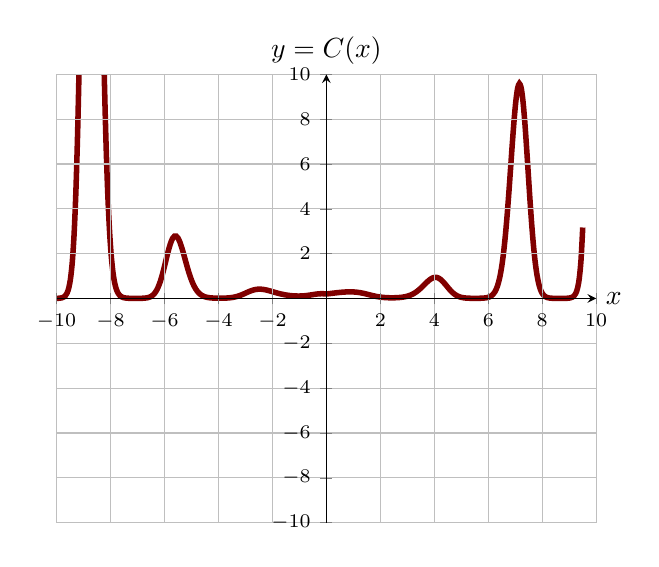
\begin{tikzpicture}
  \begin{axis}[
            domain=-10:10, ymax=10, xmax=10, ymin=-10, xmin=-10,
            axis lines =center, xlabel=$x$, ylabel={$y=C(x)$}, grid = major,
            ytick={-10,-8,-6,-4,-2,2,4,6,8,10},
            xtick={-10,-8,-6,-4,-2,2,4,6,8,10},
            yticklabels={$-10$,$-8$,$-6$,$-4$,$-2$,$2$,$4$,$6$,$8$,$10$}, 
            xticklabels={$-10$,$-8$,$-6$,$-4$,$-2$,$2$,$4$,$6$,$8$,$10$},
            ticklabel style={font=\scriptsize},
            every axis y label/.style={at=(current axis.above origin),anchor=south},
            every axis x label/.style={at=(current axis.right of origin),anchor=west},
            axis on top
          ]
          
          %\addplot [line width=2, penColor2, smooth,samples=100,domain=(-6:2)] {-2*x-3};
            \addplot [line width=2, penColor2, smooth,samples=300,domain=(-10:9.5)] {(sin(deg(2*x))+2)^abs(x)/(5*(x^2+1))};

          %\addplot[color=penColor,fill=penColor2,only marks,mark=*] coordinates{(-6,9)};
          %\addplot[color=penColor,fill=penColor2,only marks,mark=*] coordinates{(2,-7)};

          %\addplot[color=penColor2,fill=white,only marks,mark=*] coordinates{(2,-4.5)};
          %\addplot[color=penColor2,fill=white,only marks,mark=*] coordinates{(8,6)};


           

  \end{axis}
\end{tikzpicture}
\end{image}









The algebra is beyond us. \\




The formula is too difficult to manipulate with algebra.  So, we concentrate on approximations. \\ 


The function is too complicated to consider as a whole. So, we think of it in pieces - small pieces. \\






If we are only interested in approximating small pieces of the function, then we can use a replacement function that does a pretty good job of approximating this function over a small interval - a replacement that is easier to work with.

And, our favorite functions are linear functions.


$C(x)$ appears to be linear-ish on the interval $(6.6, 7.0)$. Our plan is to create a linear function that does a pretty good job of approximating $C(x)$ on the interval. Graphically, that means a tangent line around $6.8$.  We need two data for this.  We need $C(6.8)$ and $C'(6.8)$.





Out linear approximation will be $approxC(x) = C'(6.8)(x-6.8) + C(6.8)$.

Of course, it will only be useful on $(6.6, 7.0)$, if that. \\




We'll need the derivative (which Calculus will. provide): \\
\textbf{Note:} On the interval $(6.6, 7.0)$, $| x | = x$.

\[  
C'(x) = \frac{(\sin(2x)+2)^x (\ln(\sin(2x)+2) + \frac{2 x \cos(2x)}{\sin(2x)+2})}{5(x^2+1)} - \frac{2x(\sin(2x)+2)^x}{5(x^2+1)^2}
\]




That's terrible.  But we only need it for $6.8$ and we are approximating, for which decimal numbers are handy.

$C'(6.8) \approx 17.132$


$C(6.8) \approx 5.359$


That gives $approxC(x) \approx 17.132(x-6.8)+5.359$







\begin{image}
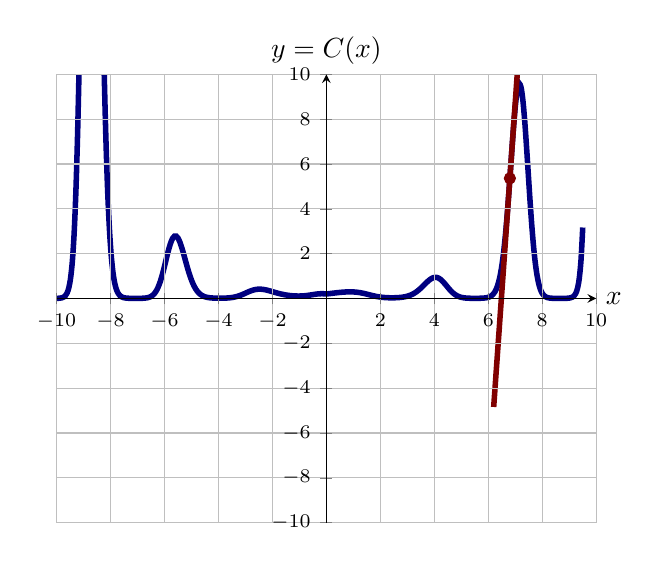
\begin{tikzpicture}
  \begin{axis}[
            domain=-10:10, ymax=10, xmax=10, ymin=-10, xmin=-10,
            axis lines =center, xlabel=$x$, ylabel={$y=C(x)$}, grid = major,
            ytick={-10,-8,-6,-4,-2,2,4,6,8,10},
            xtick={-10,-8,-6,-4,-2,2,4,6,8,10},
            yticklabels={$-10$,$-8$,$-6$,$-4$,$-2$,$2$,$4$,$6$,$8$,$10$}, 
            xticklabels={$-10$,$-8$,$-6$,$-4$,$-2$,$2$,$4$,$6$,$8$,$10$},
            ticklabel style={font=\scriptsize},
            every axis y label/.style={at=(current axis.above origin),anchor=south},
            every axis x label/.style={at=(current axis.right of origin),anchor=west},
            axis on top
          ]
          
          %\addplot [line width=2, penColor2, smooth,samples=100,domain=(-6:2)] {-2*x-3};
            \addplot [line width=2, penColor, smooth,samples=300,domain=(-10:9.5)] {(sin(deg(2*x))+2)^abs(x)/(5*(x^2+1))};

          \addplot [line width=2, penColor2, smooth,samples=100,domain=(6.2:7.2)] {17*(x-6.8)+5.36};
          \addplot[color=penColor2,fill=penColor2,only marks,mark=*] coordinates{(6.8,5.36)};

           

  \end{axis}
\end{tikzpicture}
\end{image}












That is pretty good on $(6.6, 7.0)$.






\begin{image}
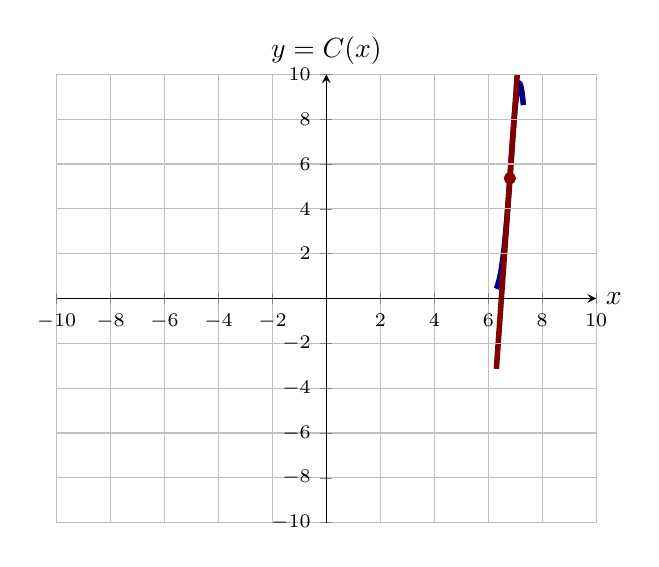
\begin{tikzpicture}
  \begin{axis}[
            domain=-10:10, ymax=10, xmax=10, ymin=-10, xmin=-10,
            axis lines =center, xlabel=$x$, ylabel={$y=C(x)$}, grid = major,
            ytick={-10,-8,-6,-4,-2,2,4,6,8,10},
            xtick={-10,-8,-6,-4,-2,2,4,6,8,10},
            yticklabels={$-10$,$-8$,$-6$,$-4$,$-2$,$2$,$4$,$6$,$8$,$10$}, 
            xticklabels={$-10$,$-8$,$-6$,$-4$,$-2$,$2$,$4$,$6$,$8$,$10$},
            ticklabel style={font=\scriptsize},
            every axis y label/.style={at=(current axis.above origin),anchor=south},
            every axis x label/.style={at=(current axis.right of origin),anchor=west},
            axis on top
          ]
          
          %\addplot [line width=2, penColor2, smooth,samples=100,domain=(-6:2)] {-2*x-3};
            \addplot [line width=2, penColor, smooth,samples=300,domain=(6.3:7.3)] {(sin(deg(2*x))+2)^abs(x)/(5*(x^2+1))};

          \addplot [line width=2, penColor2, smooth,samples=100,domain=(6.3:7.3)] {17*(x-6.8)+5.36};
          \addplot[color=penColor2,fill=penColor2,only marks,mark=*] coordinates{(6.8,5.36)};

           

  \end{axis}
\end{tikzpicture}
\end{image}







\begin{image}
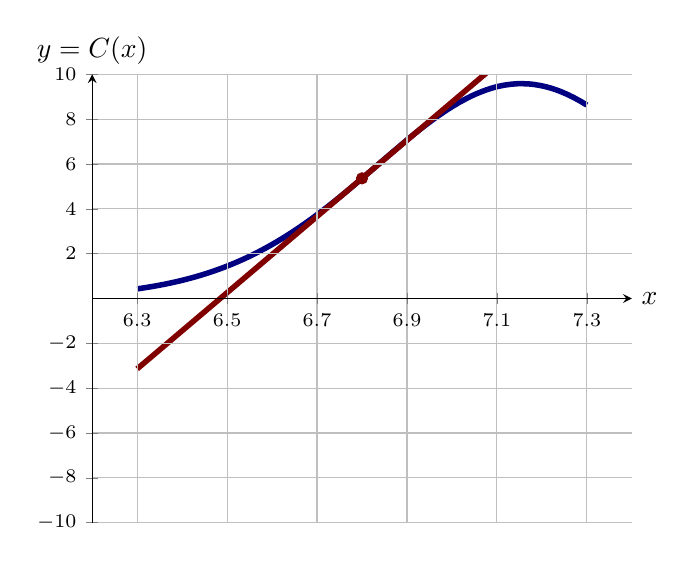
\begin{tikzpicture}
  \begin{axis}[
            domain=6.2:7.4, ymax=10, xmax=7.4, ymin=-10, xmin=6.2,
            axis lines =center, xlabel=$x$, ylabel={$y=C(x)$}, grid = major,
            ytick={-10,-8,-6,-4,-2,2,4,6,8,10},
            xtick={6.3,6.5,6.7,6.9,7.1,7.3},
            yticklabels={$-10$,$-8$,$-6$,$-4$,$-2$,$2$,$4$,$6$,$8$,$10$}, 
            xticklabels={$6.3$,$6.5$,$6.7$,$6.9$,$7.1$,$7.3$},
            ticklabel style={font=\scriptsize},
            every axis y label/.style={at=(current axis.above origin),anchor=south},
            every axis x label/.style={at=(current axis.right of origin),anchor=west},
            axis on top
          ]
          
          %\addplot [line width=2, penColor2, smooth,samples=100,domain=(-6:2)] {-2*x-3};
            \addplot [line width=2, penColor, smooth,samples=300,domain=(6.3:7.3)] {(sin(deg(2*x))+2)^abs(x)/(5*(x^2+1))};

          \addplot [line width=2, penColor2, smooth,samples=100,domain=(6.3:7.3)] {17*(x-6.8)+5.36};
          \addplot[color=penColor2,fill=penColor2,only marks,mark=*] coordinates{(6.8,5.36)};

           

  \end{axis}
\end{tikzpicture}
\end{image}








Now we can approximate $C(x) \approx approxC(x) \approx 17.132(x-6.8)+5.359$ on $(6.6, 7.0)$.  That would save a lot of time and energy and not give up too much accuracy - as long as we stay in this interval.






However, these types of functions are for later courses.  We are just trying to figure out the concept here.  So, let's bring our investigation back down to our elementary functions.





\section*{Linear Approximations}


Approximating complex functions with linear functions is an important aspect of analysis, even if it is over a small interval.







\begin{example} Square Roots



Approximate $\sqrt{4.5}$ with a decimal expansion.

\begin{explanation}

First, graph $y = s(t) = \sqrt{t}$.


\begin{image}
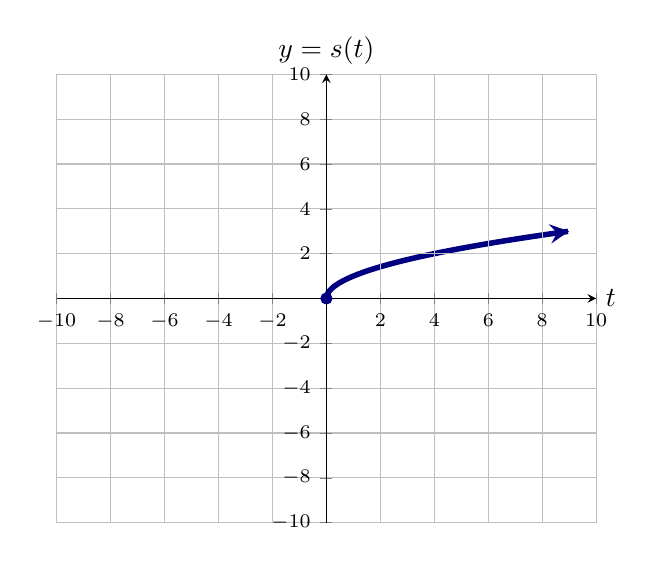
\begin{tikzpicture}
  \begin{axis}[
            domain=-10:10, ymax=10, xmax=10, ymin=-10, xmin=-10,
            axis lines =center, xlabel=$t$, ylabel={$y=s(t)$}, grid = major,
            ytick={-10,-8,-6,-4,-2,2,4,6,8,10},
            xtick={-10,-8,-6,-4,-2,2,4,6,8,10},
            yticklabels={$-10$,$-8$,$-6$,$-4$,$-2$,$2$,$4$,$6$,$8$,$10$}, 
            xticklabels={$-10$,$-8$,$-6$,$-4$,$-2$,$2$,$4$,$6$,$8$,$10$},
            ticklabel style={font=\scriptsize},
            every axis y label/.style={at=(current axis.above origin),anchor=south},
            every axis x label/.style={at=(current axis.right of origin),anchor=west},
            axis on top
          ]
          
          	
			\addplot [line width=2, penColor, smooth,samples=200,domain=(0:9),->] {sqrt(x)};
			\addplot[color=penColor,fill=penColor,only marks,mark=*] coordinates{(0,0)};
			%\addplot [line width=2, penColor2, smooth,samples=100,domain=(6.2:7.2)] {17*(x-6.8)+5.36};
			%\addplot[color=penColor2,fill=penColor2,only marks,mark=*] coordinates{(6.8,5.36)};

  \end{axis}
\end{tikzpicture}
\end{image}


$4.5$ simply doesn't work well with the square root function.  However, $4$ does and $4$ is near $4.5$.


Let's create a linear approximation to $s(t)$ at $4$.

Courtesy of Calculus: the derivative of $s(t)$ is $s'(t) = \frac{1}{2\sqrt{t}}$.

We have 

\begin{itemize}
\item $s(4) = \sqrt{4} = 2$
\item $s'(4) = \frac{1}{2\sqrt{4}} = \frac{1}{4}$
\end{itemize}



The linear approximation is $L(t) = \frac{1}{4}(t-4)+2$










\begin{image}
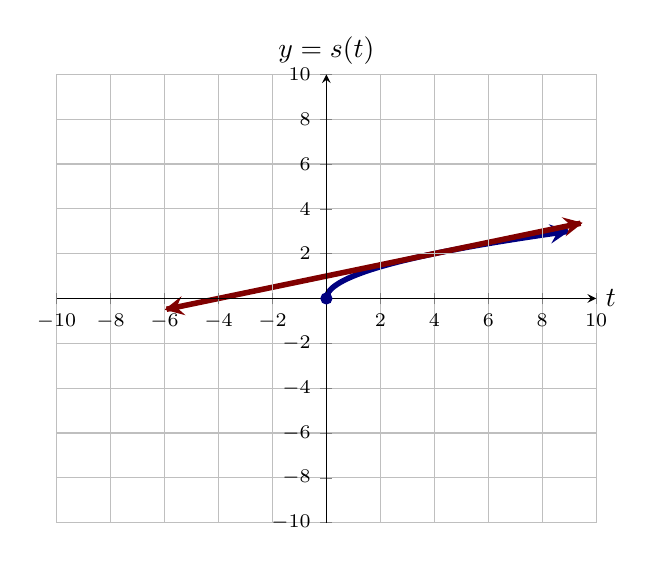
\begin{tikzpicture}
  \begin{axis}[
            domain=-10:10, ymax=10, xmax=10, ymin=-10, xmin=-10,
            axis lines =center, xlabel=$t$, ylabel={$y=s(t)$}, grid = major,
            ytick={-10,-8,-6,-4,-2,2,4,6,8,10},
            xtick={-10,-8,-6,-4,-2,2,4,6,8,10},
            yticklabels={$-10$,$-8$,$-6$,$-4$,$-2$,$2$,$4$,$6$,$8$,$10$}, 
            xticklabels={$-10$,$-8$,$-6$,$-4$,$-2$,$2$,$4$,$6$,$8$,$10$},
            ticklabel style={font=\scriptsize},
            every axis y label/.style={at=(current axis.above origin),anchor=south},
            every axis x label/.style={at=(current axis.right of origin),anchor=west},
            axis on top
          ]
          
          	
			\addplot [line width=2, penColor, smooth,samples=200,domain=(0:9),->] {sqrt(x)};
			\addplot[color=penColor,fill=penColor,only marks,mark=*] coordinates{(0,0)};
			\addplot [line width=2, penColor2, smooth,samples=200,domain=(-6:9.5),<->] {0.25*(x-4)+2};

  \end{axis}
\end{tikzpicture}
\end{image}

Now we'll use our linear approximation to get an estimate to $\sqrt{4.5} = s(4.5)$.



\[   \sqrt{4.5} \approx   \frac{1}{4}(4.5-4)+2    =   \frac{0.5}{4}+2 =    2.125   \]

Compare this to what a calculator gives: $2.121320344$.  Not bad for just a linear function.



\end{explanation}

\end{example}








\section*{Polygonal Lines}


We might even approximate a function over a wider interval, just use more linear functions (i.e. line segments).





Graph of $y = p(k) = -k^2 + 7$.




\begin{image}
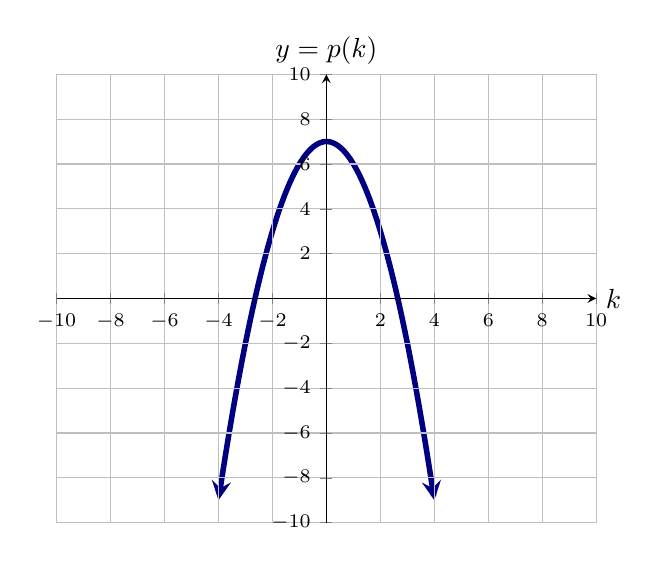
\begin{tikzpicture}
  \begin{axis}[
            domain=-10:10, ymax=10, xmax=10, ymin=-10, xmin=-10,
            axis lines =center, xlabel=$k$, ylabel={$y=p(k)$}, grid = major,
            ytick={-10,-8,-6,-4,-2,2,4,6,8,10},
            xtick={-10,-8,-6,-4,-2,2,4,6,8,10},
            yticklabels={$-10$,$-8$,$-6$,$-4$,$-2$,$2$,$4$,$6$,$8$,$10$}, 
            xticklabels={$-10$,$-8$,$-6$,$-4$,$-2$,$2$,$4$,$6$,$8$,$10$},
            ticklabel style={font=\scriptsize},
            every axis y label/.style={at=(current axis.above origin),anchor=south},
            every axis x label/.style={at=(current axis.right of origin),anchor=west},
            axis on top
          ]
          
          	
			\addplot [line width=2, penColor, smooth,samples=200,domain=(-4:4),<->] {-(x^2)+7};
			%\addplot[color=penColor,fill=penColor,only marks,mark=*] coordinates{(0,0)};
			%\addplot [line width=2, penColor2, smooth,samples=200,domain=(-6:9.5),<->] {0.25*(x-4)+2};

  \end{axis}
\end{tikzpicture}
\end{image}




Let's approximate $p(k) = -k^2+7$ with five linear functions, corresponding to five tangent lines tangent where $k=-2, -1, 0, 1, 2$.

$p(k)$ is a quadratic function, therefore, we know that $p'(k) = -2k$.  This will get us rate of change or slope.  Together with the point of tangency, we can get a linear model of $p(k)$.


\begin{model}

\begin{itemize}
\item $p(-2) = 3$ and $p'(-2) = 4$ give $p(k) \approx 4(k+2)+3$
\item $p(-1) = 6$ and $p'(-1) = 2$ give $p(k) \approx \answer{2(k+1)+6}$
\item $p(0) = 7$ and $p'(0) = 0$   give $p(k) \approx \answer{7}$
\item $p(1) = 6$ and $p'(1) = -2$   give  $ p(k) \approx \answer{-2(k-1)+6}$
\item $p(2) = 3$ and $p'(2) = -44$   give $p(k) \approx -4(k-2)+3$
\end{itemize}

\end{model}










\begin{image}
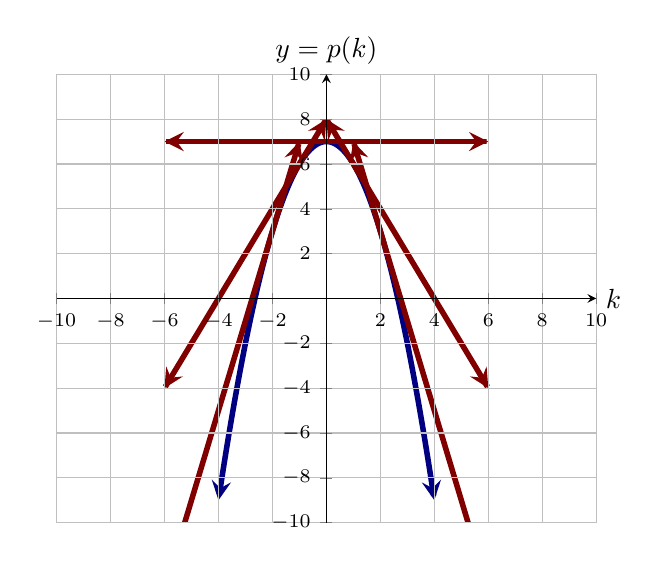
\begin{tikzpicture}
  \begin{axis}[
            domain=-10:10, ymax=10, xmax=10, ymin=-10, xmin=-10,
            axis lines =center, xlabel=$k$, ylabel={$y=p(k)$}, grid = major,
            ytick={-10,-8,-6,-4,-2,2,4,6,8,10},
            xtick={-10,-8,-6,-4,-2,2,4,6,8,10},
            yticklabels={$-10$,$-8$,$-6$,$-4$,$-2$,$2$,$4$,$6$,$8$,$10$}, 
            xticklabels={$-10$,$-8$,$-6$,$-4$,$-2$,$2$,$4$,$6$,$8$,$10$},
            ticklabel style={font=\scriptsize},
            every axis y label/.style={at=(current axis.above origin),anchor=south},
            every axis x label/.style={at=(current axis.right of origin),anchor=west},
            axis on top
          ]
          
          	
			\addplot [line width=2, penColor, smooth,samples=200,domain=(-4:4),<->] {-(x^2)+7};
			%\addplot[color=penColor,fill=penColor,only marks,mark=*] coordinates{(0,0)};
			\addplot [line width=2, penColor2, smooth,samples=200,domain=(-6:-1),<->] {4*(x+2)+3};
			\addplot [line width=2, penColor2, smooth,samples=200,domain=(-6:0),<->] {2*(x+1)+6};
			\addplot [line width=2, penColor2, smooth,samples=200,domain=(-6:6),<->] {7};
			\addplot [line width=2, penColor2, smooth,samples=200,domain=(0:6),<->] {-2*(x-1)+6};
			\addplot [line width=2, penColor2, smooth,samples=200,domain=(1:6),<->] {-4*(x-2)+3};

  \end{axis}
\end{tikzpicture}
\end{image}



It looks like maybe these will approximate $p(k)$ on $(-3, 3)$.








\begin{image}
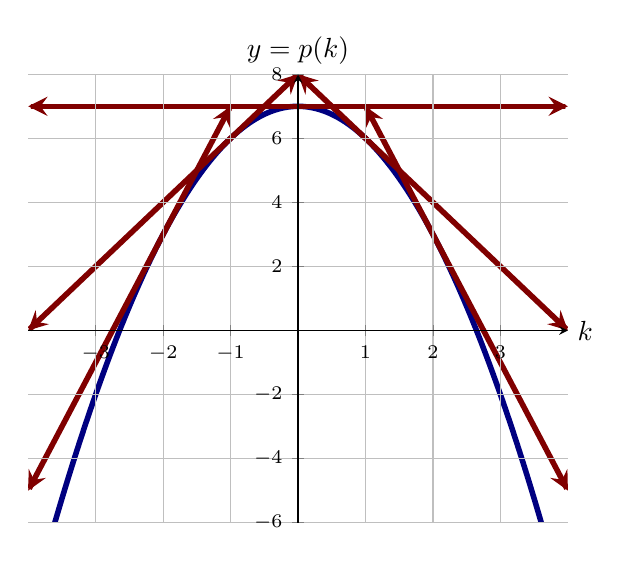
\begin{tikzpicture}
  \begin{axis}[
            domain=-4:4, ymax=8, xmax=4, ymin=-6, xmin=-4,
            axis lines =center, xlabel=$k$, ylabel={$y=p(k)$}, grid = major,
            ytick={-6,-4,-2,2,4,6,8},
            xtick={-3,-2,-1,1,2,3},
            yticklabels={$-6$,$-4$,$-2$,$2$,$4$,$6$,$8$}, 
            xticklabels={$-3$,$-2$,$-1$,$1$,$2$,$3$},
            ticklabel style={font=\scriptsize},
            every axis y label/.style={at=(current axis.above origin),anchor=south},
            every axis x label/.style={at=(current axis.right of origin),anchor=west},
            axis on top
          ]
          
            
      \addplot [line width=2, penColor, smooth,samples=200,domain=(-4:4),<->] {-(x^2)+7};
      %\addplot[color=penColor,fill=penColor,only marks,mark=*] coordinates{(0,0)};
      \addplot [line width=2, penColor2, smooth,samples=200,domain=(-4:-1),<->] {4*(x+2)+3};
      \addplot [line width=2, penColor2, smooth,samples=200,domain=(-4:0),<->] {2*(x+1)+6};
      \addplot [line width=2, penColor2, smooth,samples=200,domain=(-4:4),<->] {7};
      \addplot [line width=2, penColor2, smooth,samples=200,domain=(0:4),<->] {-2*(x-1)+6};
      \addplot [line width=2, penColor2, smooth,samples=200,domain=(1:4),<->] {-4*(x-2)+3};

  \end{axis}
\end{tikzpicture}
\end{image}



















Now we need domains for each piece.  We'll decide the domains by locating the intersections of the lines.




$\blacktriangleright$  Intersection of $4(k+2)+3$ and $2(k+1)+6$.

\begin{procedure}

$4(k+2)+3 = 2(k+1)+6 $

$4k + 8 + 3 = \answer{2k + 2 + 6}$

$2k = \answer{-3}$

$k=-\frac{3}{2}$

\end{procedure}


$\blacktriangleright$  Intersection of $2(k+1)+6$ and $7$.

\begin{procedure}

$2(k+1)+6 = 7$

$2k + 2 + 6 = 7$

$2k = \answer{-1}$

$k = -\frac{1}{2}$

\end{procedure}




$\blacktriangleright$  By symmetry we can see that the other two intersections happen when $k = \frac{1}{2}$  and $k = \frac{3}{2}$.



Our approximating piecewise linear function is 



\[
p(k) \approx L(k) = 
\begin{cases}
  4(k+2)+3       &          \text{ on } \,     \left(-3, -\frac{3}{2}\right]   \\
  2(k+1)+6       &          \text{ on } \,     \left(-\frac{3}{2}, -\frac{1}{2}\right]   \\
  7              &          \text{ on } \,     \left(-\frac{1}{2}, \frac{1}{2}\right]   \\
  -2(k-1)+6      &          \text{ on } \,     \left(\frac{1}{2}, \frac{3}{2}\right]   \\
  -4(k-2)+3      &          \text{ on } \,     \left(\frac{3}{2}, 3\right)   
\end{cases}
\]










\begin{image}
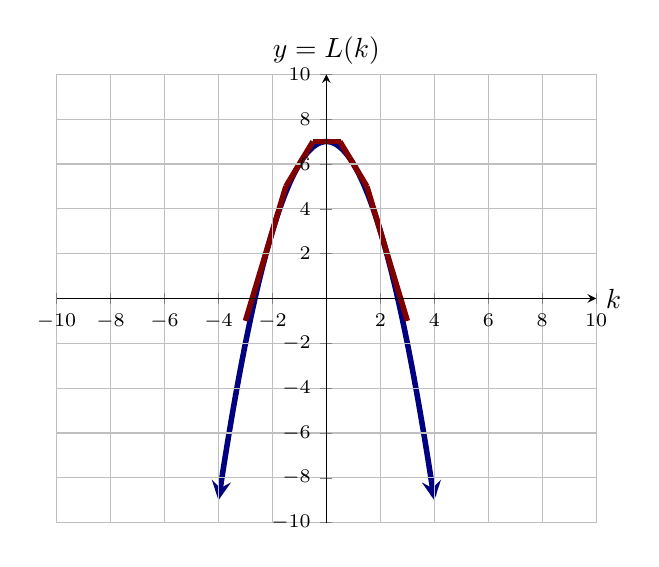
\begin{tikzpicture}
  \begin{axis}[
            domain=-10:10, ymax=10, xmax=10, ymin=-10, xmin=-10,
            axis lines =center, xlabel=$k$, ylabel={$y=L(k)$}, grid = major,
            ytick={-10,-8,-6,-4,-2,2,4,6,8,10},
            xtick={-10,-8,-6,-4,-2,2,4,6,8,10},
            yticklabels={$-10$,$-8$,$-6$,$-4$,$-2$,$2$,$4$,$6$,$8$,$10$}, 
            xticklabels={$-10$,$-8$,$-6$,$-4$,$-2$,$2$,$4$,$6$,$8$,$10$},
            ticklabel style={font=\scriptsize},
            every axis y label/.style={at=(current axis.above origin),anchor=south},
            every axis x label/.style={at=(current axis.right of origin),anchor=west},
            axis on top
          ]
          
          	
			\addplot [line width=2, penColor, smooth,samples=200,domain=(-4:4),<->] {-(x^2)+7};
			%\addplot[color=penColor,fill=penColor,only marks,mark=*] coordinates{(0,0)};
			\addplot [line width=2, penColor2, smooth,samples=200,domain=(-3:-1.5)] {4*(x+2)+3};
			\addplot [line width=2, penColor2, smooth,samples=200,domain=(-1.5:-0.5)] {2*(x+1)+6};
			\addplot [line width=2, penColor2, smooth,samples=200,domain=(-0.5:0.5)] {7};
			\addplot [line width=2, penColor2, smooth,samples=200,domain=(0.5:1.5)] {-2*(x-1)+6};
			\addplot [line width=2, penColor2, smooth,samples=200,domain=(1.5:3)] {-4*(x-2)+3};

  \end{axis}
\end{tikzpicture}
\end{image}




Pretty good.











\begin{image}
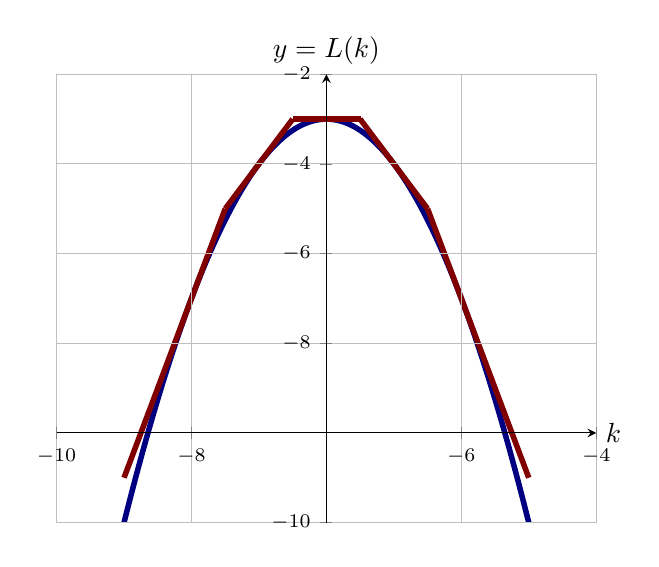
\begin{tikzpicture}
  \begin{axis}[
            domain=-4:4, ymax=8, xmax=4, ymin=-2, xmin=-4,
            axis lines =center, xlabel=$k$, ylabel={$y=L(k)$}, grid = major,
            ytick={-2,2,4,6,8},
            xtick={-4,-2,2,4},
            yticklabels={$-10$,$-8$,$-6$,$-4$,$-2$,$2$,$4$,$6$,$8$,$10$}, 
            xticklabels={$-10$,$-8$,$-6$,$-4$,$-2$,$2$,$4$,$6$,$8$,$10$},
            ticklabel style={font=\scriptsize},
            every axis y label/.style={at=(current axis.above origin),anchor=south},
            every axis x label/.style={at=(current axis.right of origin),anchor=west},
            axis on top
          ]
          
          	
			\addplot [line width=2, penColor, smooth,samples=200,domain=(-4:4),<->] {-(x^2)+7};
			%\addplot[color=penColor,fill=penColor,only marks,mark=*] coordinates{(0,0)};
			\addplot [line width=2, penColor2, smooth,samples=200,domain=(-3:-1.5)] {4*(x+2)+3};
			\addplot [line width=2, penColor2, smooth,samples=200,domain=(-1.5:-0.5)] {2*(x+1)+6};
			\addplot [line width=2, penColor2, smooth,samples=200,domain=(-0.5:0.5)] {7};
			\addplot [line width=2, penColor2, smooth,samples=200,domain=(0.5:1.5)] {-2*(x-1)+6};
			\addplot [line width=2, penColor2, smooth,samples=200,domain=(1.5:3)] {-4*(x-2)+3};

  \end{axis}
\end{tikzpicture}
\end{image}



Linear approximations do better on straight parts of the graph rather than parts with more curve to them.  Calculus will give us a way of measuring this curvature.











\begin{center}
\textbf{\textcolor{green!50!black}{ooooo-=-=-=-ooOoo-=-=-=-ooooo}} \\

more examples can be found by following this link\\ \link[More Examples of Approximate Behavior]{https://ximera.osu.edu/csccmathematics/precalculus1/precalculus1/nearEquivalentBehavior/examples/exampleList}

\end{center}



\end{document}
